\documentclass{math201}

\usepackage[backref]{hyperref} 
\hypersetup{hidelinks}
\usepackage{bookmark}

% =============================================
% Part 0 信息
% =============================================

\mathsetup{
  % 学生姓名
  student = {},
  % 学号
  student-id = {},
  % 院系
  experiment = {CPU定时器0中断实验},
  % 专业年级
  discipline = {集成电路设计与集成系统},
  % 日期
  date = {\today},
}

\begin{document}

% =============================================
% Part 1  封面
% =============================================

\makecover

% =============================================
% Part 2 主文档
% =============================================

\section{实验内容}

利用CPU定时器0的周期中断来控制LED灯的闪烁。
CPU定时器0每次定时时间到,实现指示灯的定时闪烁,这种方法比软件循环延时更能实现精确的定时。

\section{实验原理}

\subsection{F2812的CPU定时器}

X281x芯片内部具有3个32位的CPU定时器 -- Timer0, Timer1 和 Timer2。
其中,CPU 定时器1和2被系统保留,用于实时操作系统,例如DSP BIOS;只有CPU定时器0可以供用户使用。

\subsection{F2812定时器的控制方法}

\begin{figure}[H]  
    \centering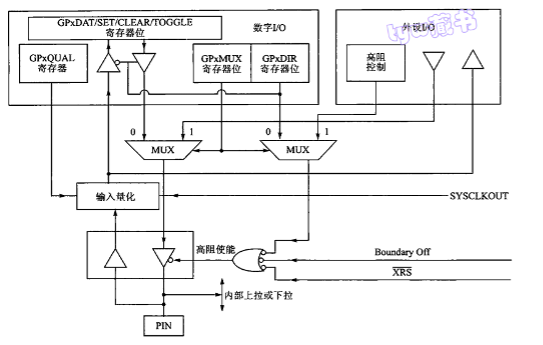
\includegraphics[width=0.8\linewidth]{Picture1.jpg}  
    \caption{CPU定时器内部结构}     
    \label{img01}   
\end{figure}

从图1可以看到CPU 定时器的几个寄存器:
32位的定时器周期寄存器 PRDH:PRD,
32 位的计数器寄存器 TIMH:TIM,
16位的定时器分频器寄存器TD-DRH:TDDR,
16位的预定标计数器寄存器 PSCH:PSC。
这里第 1 次遇到“XH:X”形式表示存器的方式。因为 X28IxDSP 的寄存器都是 16 位的,但是 CPU 定时器是 32 位的,,例如定时器周期寄存器、定时器计数器寄存器。
可以用2个16 位的寄存器XH和又来表示32位的寄存器,其中 XH表示高16位,而X表示低16位。

\subsection{F2812的中断结构和对中断的处理流程}

\begin{figure}[H]  
    \centering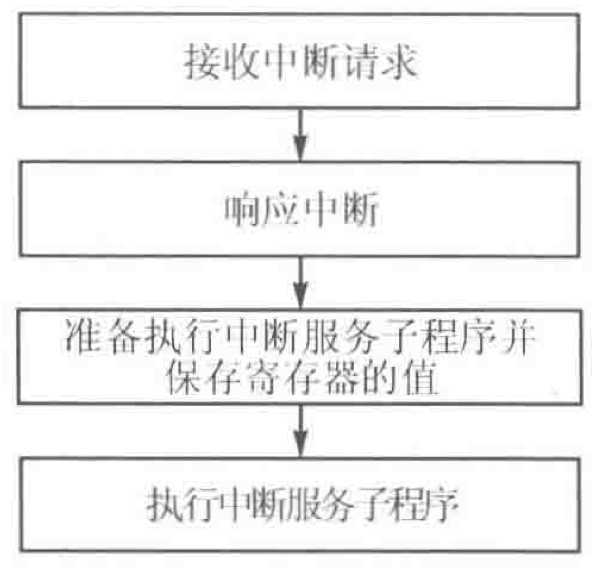
\includegraphics[width=0.8\linewidth]{Picture2.png}  
    \caption{CPU处理中断的4个步骤}     
    \label{img02}   
\end{figure}

X2812 的中断主要有两种方式触发:
一种是在软件中写指令,例如 INTR、OR IFR或者 TRAP 指令;
另一种是硬件方式触发,例如来自片内外设或者外围设备的中断信号,表示某个事件已经发生。
无论是软件中断还是硬件中断,都可以归结为可屏蔽中断和不可屏蔽中断。

所谓可屏蔽中断就是这些中断可以用软件加以屏蔽或者解除屏蔽。X2812片内外设所产生的中断都是可屏蔽中断,每一个中断都可以通过相应寄存器的中断使能位来禁止或者使能该中断。

不可屏蔽中断就是这些中断是不可以被屏蔽的,一旦中断申请信号发出,CPU 必须无条件的立即去响应该中断并执行相应的中断服务子程序。
X281x的不可屏蔽中断主要包括软件中断(INTR指令和 TRAP指令等)、硬件中断 NMI、非法指令陷阱以及硬件复位中断。

X2812的CPU 按照图2所示的4个步骤来处理中断。
首先由外设或者其他方式向 CPU 提出中断请求,然后如果这个中断是可屏蔽中断,CPU便会去检查这个中断的使能情况,再决定是否响应该中断;如果这个中断是不可屏蔽中断,则CPU便会立即响应该中断。
接着,CPU 会完整地执行完当前指令,为了记住当前主程序的状态,CPU 必须要做一些准备工作,例如将 ST0、T、AH、AL、PC 等寄存器的内容保存到堆栈中,以便自动保存主程序的大部分内容。
在准备工作做完之后,CPU 就取回中断向量,开始执行中断服务子程序。当然,处理完相应的中断事件之后,CPU 就回到原来主程序暂停的地方,恢复各个寄存器的内容,继续执行主程序。

\section{实验步骤}

\subsection{编写代码}

修改 main.c

\inputminted[
    frame=lines,
    framesep=2mm,
    baselinestretch=1.2,
    fontsize=\small,
    linenos
]{C++}{code/main.c}

修改 common\_files/DSP2812\_resources/DSP281x\_DefaultIsr.c

\inputminted[
    frame=lines,
    framesep=2mm,
    baselinestretch=1.2,
    fontsize=\small,
    linenos
]{C++}{code/DSP281x_DefaultIsr.c}

为了简化开发过程,可以在lab4项目的基础上进行修改。但需要注意的是,请删除lab4项目中的num.h文件,否则会导致意想不到编译错误。

\subsection{下载运行、实验现象}

编译下载运行,实验现象如下,可以看到LED灯每隔一秒闪烁一次,循环运行。

\begin{figure}[H]  
  \centering\includegraphics[width=0.8\linewidth]{led1.jpg}  
  \caption{实验现象1}      
\end{figure}

\begin{figure}[H]  
  \centering\includegraphics[width=0.8\linewidth]{led2.jpg}  
  \caption{实验现象2}      
\end{figure}

\begin{figure}[H]  
  \centering\includegraphics[width=0.8\linewidth]{led3.jpg}  
  \caption{实验现象3}      
\end{figure}

\begin{figure}[H]  
  \centering\includegraphics[width=0.8\linewidth]{led4.jpg}  
  \caption{实验现象4}      
\end{figure}

\section{实验小结}

本实验的目的是利用CPU定时器0的周期中断来控制LED灯的闪烁,实验的原理是通过设置CPU定时器的寄存器和中断向量来实现定时中断的响应和处理,实验的步骤是编写相应的C代码,修改main.c和DSP281x\_DefaultIsr.c文件,实验的现象是观察LED灯每隔一秒闪烁一次,循环运行。

\end{document}
